\documentclass[12pt, a4 paper]{article}
% Set target color model to RGB
\usepackage[inner=2.0cm,outer=2.0cm,top=2.5cm,bottom=2.5cm]{geometry}
\usepackage{setspace}
\usepackage[rgb]{xcolor}
\usepackage{environ}
\usepackage{verbatim}
\usepackage{subcaption}
\usepackage{outlines}
\usepackage{enumitem}
\usepackage{amsgen,amsmath,amstext,amsbsy,amsopn,tikz,amssymb,tkz-linknodes}
\usepackage{fancyhdr}
\usepackage{pgfplots}
\usepackage{mathtools}
\usepackage[colorlinks=true, urlcolor=blue,  linkcolor=blue, citecolor=blue]{hyperref}
\usepackage[colorinlistoftodos]{todonotes}
\usepackage{rotating}

\linespread{1.6} % Double Line Spacing
\usetikzlibrary{arrows.meta,intersections,calc}

\hypersetup{%
pdfauthor={Vignesh Ravibaskar},%
pdfcreator={PDFLaTeX},%
pdfproducer={PDFLaTeX},%
}

% Our custom enumerate labelling, just making the outlines bold basically
\setlist[enumerate,1]{label=\textbf{\arabic*}}
\setlist[enumerate,2]{label=\textbf{({\alph*})}}
\setlist[enumerate,3]{label=\textbf{({\roman*})}}

\title{Differentiation}
\author{Derek, Vignesh}
\date{2020}

\newcommand{\comm}[1]{}
\NewEnviron{answer}{\vspace{3mm} \\ \color{blue} {\BODY} \color{black}}
%\NewEnviron{answer}{\color{blue} \comm{\BODY} \color{black}} % Use this method to hide all answers

\begin{document}

\maketitle

\textbf{DIFFERENTIATION [80 Marks]}
\begin{outline}[enumerate]

 \1 Differentiate with respect to $x$ the following: %Question 1

 \2 $\ln (\ln ({x^2}))$\hfill[2]
 \begin{answer}
  Recall that $\frac{\mathrm{d}}{\mathrm{d}x}\ln(x^2)=\frac{2}{x}$
  \begin{align*}
   \frac{\mathrm{d}}{\mathrm{d}x}\ln (\ln ({x^2})) = \frac{2}{x\ln ({x^2})}
  \end{align*}
 \end{answer}

 \2 $4^{\cos 4x}$\hfill[2]
 \begin{answer}
  Recall that you can express $4^{\cos4x}$ as $\mathrm{e}^{\ln4cos4x}$
  \begin{align*}
   \frac{\mathrm{d}}{\mathrm{d}x}4^{\cos 4x} & =\frac{\mathrm{d}}{\mathrm{d}x}\mathrm{e}^{\ln4cos4x} \\
                                             & = -8\ln2 \cdot \sin4x \cdot \mathrm{e}^{\ln4cos4x}    \\
                                             & = -8\ln2 \cdot \sin4x \cdot 4^{\cos4x}
  \end{align*}
 \end{answer}

 \2 $\tan ^{ - 1}(xy)$\hfill[2]
 \begin{answer}
  Recall that differentiating $xy$ wrt $x$ gives you $y+x\frac{\mathrm{d}y}{\mathrm{d}x}$
  \begin{align*}
   \frac{\mathrm{d}}{\mathrm{d}x}\tan ^{ - 1}(xy) & = \frac{y+x\frac{\mathrm{d}y}{\mathrm{d}x}}{1+(xy)^2}
  \end{align*}
 \end{answer}

 \2 $\dfrac{{{x^2}}}{3} - \dfrac{{{y^2}}}{4} = 1$\hfill[2]
 \begin{answer}
  \begin{align*}
   \frac{\mathrm{d}}{\mathrm{d}x}\left[\dfrac{{{x^2}}}{3} - \dfrac{{{y^2}}}{4}\right] = \frac{2}{3}x-\frac{1}{2}y\cdot\frac{\mathrm{d}y}{\mathrm{d}x} = 0
  \end{align*}
 \end{answer}

 \1 Solve the following differential equations: %Question 2
 \begin{answer}
  For this section, we will collect similar terms ($\mathrm{d}y, y$) terms on the same side before integrating them respectively
 \end{answer}

 \2 $\dfrac{{{\rm{d}}y}}{{{\rm{d}}x}} = 2y,\;y = 1{\textrm{ when }}\,x = 1$ \hfill[2]
 \begin{answer}
  \begin{align*}
   \frac{\mathrm{d}y}{y} & = 2\mathrm{d}x                     \\
   \ln|y|                & = 2x+C \implies C=\ln(1)-2(1) = -2 \\
   y                     & = \mathrm{e}^{2x-2}
  \end{align*}
 \end{answer}

 \2 $\dfrac{{{\rm{d}}x}}{{{\rm{d}}t}} = 4({x^2} + x + 1)$ \hfill[3]
 \begin{answer}
  \begin{align*}
   \frac{\mathrm{d}x}{x^2+x+1}                                & = 4\mathrm{d}t \\
   \frac{\mathrm{d}x}{(x+\frac{1}{2})^2+(\frac{\sqrt3}{2})^2} & = 4\mathrm{d}t \\
   \frac{2}{\sqrt3}\tan^{-1}\left(\frac{2x+1}{\sqrt3}\right)  & = 4t + C       \\
   x = \frac{1}{2}\left[\sqrt3\tan\left(\frac{8\sqrt3}{3}t + C\right)-1\right]
  \end{align*}
 \end{answer}

 \2 $\dfrac{{{\rm{d}}y}}{{{\rm{d}}x}} = \dfrac{{ - {\mathrm{e}^{ - 3x}}}}{{3y}}$ \hfill[3]
 \begin{answer}
  \begin{align*}
   y\,\mathrm{d}y & = -\frac{\mathrm{e}^{-3x}}{3} \mathrm{d}x \\
   \frac{1}{2}y^2 & = \frac{1}{9}\mathrm{e}^{-3x} + C         \\
   y              & = \sqrt{\frac{2}{9}\mathrm{e}^{-3x} + C}
  \end{align*}
 \end{answer}

 \1 The parametric equations of curve C are: \[x = t + 1,\;y = \frac{1}{{{t^2} + 2t + 2}}{\textrm{ where }} - 3 \leq t \leq 1.\] %Question 3

 \2 Find the Cartesian equation of $C$. \hfill[2]
 \begin{answer}
  Notice that $t^2+2t+2 = (t+1)^2 = x^2\implies$ The Cartesian equation is $y=\frac{1}{x^2}$
 \end{answer}

 \2 Find the equation of the tangent to the curve $C$ when $t=2$.\hfill[3]
 \begin{answer}
  Recall that for a parametric equation, $\frac{\mathrm{d}y}{\mathrm{d}x}=\frac{\mathrm{d}y}{\mathrm{d}t}\div\frac{\mathrm{d}x}{\mathrm{d}t}$. However, it is much simpler to find $\frac{\mathrm{d}y}{\mathrm{d}x}$ directly
  \begin{align*}
   \frac{\mathrm{d}y}{\mathrm{d}x}                    & = -\frac{2}{x^3}             \\
   \left.\frac{\mathrm{d}y}{\mathrm{d}x}\right|_{t=2} & = -\frac{2}{2+1}             \\
                                                      & = -\frac{2}{3}               \\\\
   y-y|_{t=2}                                         & = -\frac{2}{3}(x-3)          \\
   y - \frac{1}{9}                                    & = -\frac{2}{3}(x-3)          \\
   \implies y                                         & = -\frac{2}{3}x+2\frac{1}{9}
  \end{align*}
 \end{answer}

 \1 Two variables $x$ and $y$ vary with time $t$ in minutes and are connected by the equation $\sin (xy) = \frac{1}{2}$. Given that $x$ increases at a rate of 3 units per minute, find the (maximum possible) rate of decrease of $y$ when $y = 1$. \hfill[4] %Question 4
 \begin{answer}
  Recall that differentiating $xy$ wrt $x$ gives you $y+x\frac{\mathrm{d}y}{\mathrm{d}x}$. Therefore, we will first differentiate $\sin (xy) = \frac{1}{2}$ wrt $x$.
  \begin{align*}
   \frac{\mathrm{d}}{\mathrm{d}x}\sin (xy)  & = \left(y+x\frac{\mathrm{d}y}{\mathrm{d}x}\right)\cos(xy) = 0           \\
   \implies \frac{\mathrm{d}y}{\mathrm{d}x} & = -\frac{y}{x}                                                          \\\\
   \frac{\mathrm{d}y}{\mathrm{d}t}          & = \frac{\mathrm{d}y}{\mathrm{d}x} \cdot \frac{\mathrm{d}x}{\mathrm{d}t} \\
                                            & = -\frac{3y}{x}                                                         \\
  \end{align*}
  To get the maximum rate of decrease, we find the minimum value of $x$
  \begin{align*}
   x|_{y=1}                                                                      & = \arcsin\left(\frac{1}{2}\right)\div 1 = \frac{\pi}{6} + 2k\pi \quad\textrm{OR}\quad \frac{5\pi}{6} + 2k\pi, k\in\mathbb{Z} \\
   \left.\frac{\mathrm{d}y}{\mathrm{d}t}\right|_{x=\frac{\pi}{6}, y=\frac{1}{2}} & = -\frac{9}{\pi}
  \end{align*}
  The maximum rate of decrease is $\frac{9}{\pi}$ units per minute.
 \end{answer}

 \1 The parametric equations of curve C are: \[x = 1 + {\mathrm{e}^{ - at}},\;y = {\mathrm{e}^{at}} + {\mathrm{e}^{ - at}}\;{\textrm{ where }}t \geq 0.\] %Question 5

 \2  Sketch $C$, including all stationary points and asymptotes where applicable.\hfill[2]
 \begin{answer}
  \color{black}
  \begin{tikzpicture}
   \begin{axis}[
     axis lines = center,
     xlabel = $x$,
     ylabel = $y$,
     xmin = 0, xmax = 2,
     ymin = 0, ymax = 10,
     legend pos=outer north east
    ]
    \addplot [
     domain=0:5,
     samples=100,
     color=blue,
    ]
    ({1+e^(-x)},
    {e^x-e^(-x)});
    \addlegendentry{$(1 + {\mathrm{e}^{ - at}}, {\mathrm{e}^{at}} + {\mathrm{e}^{ - at}})$}

    \addplot[black, mark=*, only marks] coordinates {(1,0)};
    \node[label={180:{$x=1$}}] at (axis cs:1,2) {};
    \addplot[mark=none, black, ultra thick,dotted] coordinates {(1,0) (1,12)};

    \addplot[black, mark=*, only marks] coordinates {(0,0)};
    \node[label={0:{$y=0$}}] at (axis cs:0.5,0.5) {};
   \end{axis}
  \end{tikzpicture}

 \end{answer}

 \2 Find the equation of the normal to the curve $C$ at $t = \frac{\ln{2}}{{2a}}$.\hfill[3]
 \begin{answer}
  Recall that for a parametric equation, $\frac{\mathrm{d}y}{\mathrm{d}x}=\frac{\mathrm{d}y}{\mathrm{d}t}\div\frac{\mathrm{d}x}{\mathrm{d}t}$. Furthermore, the gradient of the normal at a given point is equal to $-[\frac{\mathrm{d}y}{\mathrm{d}x}]^{-1}$ at that point
  \begin{align*}
   \frac{\mathrm{d}y}{\mathrm{d}x}=\frac{a\mathrm{e}^{at}-a\mathrm{e}^{-at}}{-a\mathrm{e}^{-at}} = 1-\mathrm{e}^{2at}
  \end{align*}
  We will now find the values for $\frac{\mathrm{d}y}{\mathrm{d}x}, x, y$ when $t=\frac{\ln2}{2a}$ to get the equation of the normal
  \begin{align*}
   \left.\frac{\mathrm{d}y}{\mathrm{d}x}\right|_{t=2}     & = -1                                      \\
   (x,y)|_{t=2}                                           & = (1+\frac{\sqrt2}{2}, \frac{3\sqrt2}{2}) \\
   \implies \textrm{Eqn Normal:}\quad y-\frac{3\sqrt2}{2} & = (x-1-\frac{\sqrt2}{2})                  \\
   y                                                      & = x-1+\sqrt2
  \end{align*}
 \end{answer}

 \2 What can be said about the normals to the curve $C$ as $t$ gets large?\hfill[1]
 \begin{answer}
  As $t\rightarrow\infty$, $\mathrm{e^{2at}}\rightarrow\infty$, thus, $-[\frac{\mathrm{d}y}{\mathrm{d}x}]^{-1} = -\frac{1}{1-\mathrm{e}^{2at}}\rightarrow0\implies$ the normals become parallel to the $x$-axis
 \end{answer}


 \1 A boy throws a rock in the air. It is launched at an angle $\theta$ to the horizontal ground, where $0 < \theta  < \frac{\pi }{2}$. As shown in the diagram, its position in the air $(x,y)$, where $x$ is the horizontal position and $y$ is the vertical position, is approximated by: \[x = (20\cos \theta )t,\,\;y = (20\sin \theta )t - 5{t^2},\]where $t$ is the time in seconds.
 \[
  \begin{tikzpicture}
   \begin{axis}[
     axis lines = center,
     xlabel = $x$,
     ylabel = $y$,
     xmin = 0, xmax=4.5,
     ymin = 0, ymax=4.5,
     xticklabels = {,,},
     yticklabels = {,,},
     legend pos=north east
    ]
    \addplot [
     domain=0:3,
     samples=100,
     color=blue,
    ]
    {x-0.2*x^2};
    \node[label] at (axis cs:0.5,0.23) {$\theta$};
    \addlegendentry{Path of stone};
   \end{axis}
   \draw[->,very thick] (0,0) -- (2,2);
   \draw[thick] (0:0.5) arc (0.5:45:0.5);
  \end{tikzpicture}
 \]

 \2 Find, in terms of $\theta$,

 \3 The time taken for the toy plane to hit the ground;\hfill[2]
 \begin{answer}
  When the toy plane hits the ground, $y=0$
  \begin{align*}
   (20\sin \theta )t - 5{t^2} = -5t(t-4\sin\theta) & = 0                                   \\
   \implies t                                      & = 0 \quad\textrm{OR}\quad 4\sin\theta
  \end{align*}
  It takes $(4\sin\theta)$s for the toy plane to hit the ground
 \end{answer}

 \3 The maximum height reached by the toy plane;\hfill[2]
 \begin{answer}
  Note that $y(t)$ is symmetrical about the centre $t=2\sin\theta$ and thus, it is at the maximum at this time.
  \begin{align*}
   y|_{t=2\sin\theta} = (20\sin\theta)\cdot2\sin\theta - 5(2\sin\theta)^2 = 20\sin^2\theta
  \end{align*}
  The maximum height is $(20\sin^2\theta)$ units.
 \end{answer}

 \3 The horizontal distance travelled by the toy plane.\hfill[2]
 \begin{answer}
  The horizontal distance is equal to the $x$ value when $t=4\sin\theta$ as we found in \textbf{(a)(i)}
  \begin{align*}
   x|_{t=4\sin\theta} = (20\cos\theta)\cdot4\sin\theta = 40\sin2\theta
  \end{align*}
  The maximum horizontal distance is $(40\sin2\theta)$ units.
 \end{answer}

 \2 Find the angle $\theta$ at which the toy plane should be thrown to attain the maximum horizontal distance.\hfill[2]
 \begin{answer}
  Intuitively, we assume that $\theta=45^\circ$ but let us verify this.
  \begin{align*}
   \frac{\mathrm{d}x}{\mathrm{d}\theta}     & = 80\cos2\theta   \\
   \frac{\mathrm{d}^2x}{\mathrm{d}\theta^2} & = -160\sin2\theta \\
  \end{align*}
  When $\frac{\mathrm{d}x}{\mathrm{d}\theta}=0$, $\theta=45^\circ$ and $\frac{\mathrm{d}^2x}{\mathrm{d}\theta^2}=-160<0\implies x$ is at a maximum
 \end{answer}

 \1 A hopper in a butter processing factory is used to store pre-processed butter before it is discharged to the next stage of the manufacturing process. One such hopper is designed with the dimensions as follows: %Question 7
 \[
  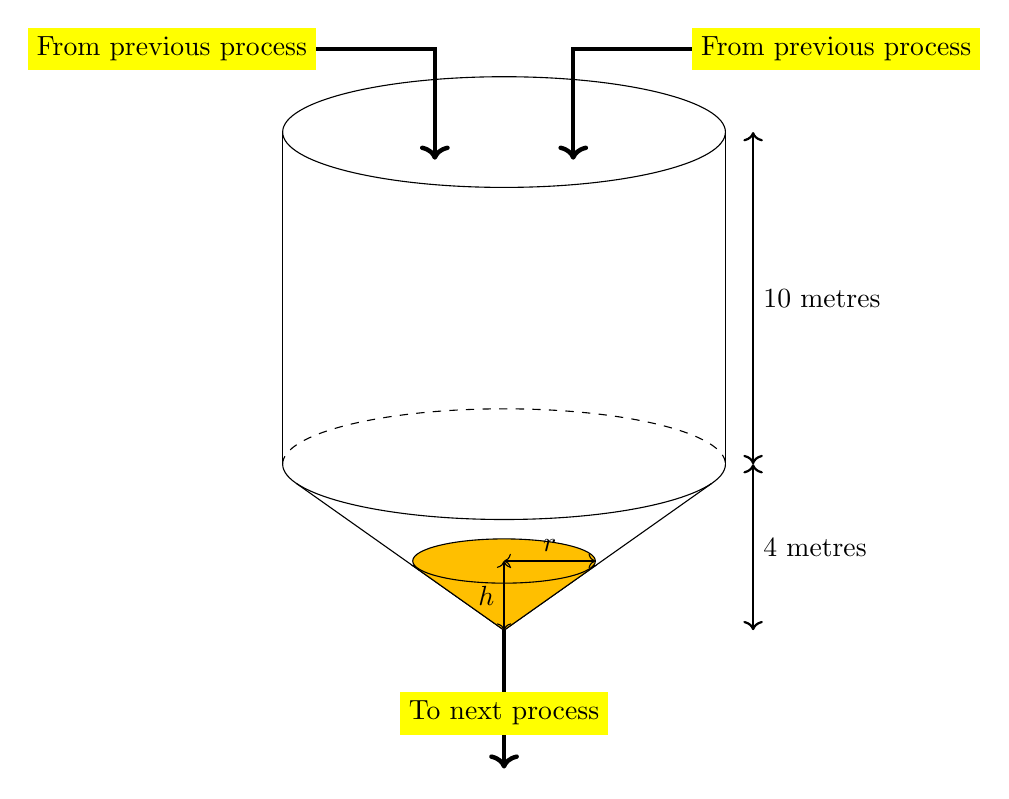
\begin{tikzpicture}
   \draw (0,0) ellipse (80pt and 20pt); %Begin Cylinder
   \draw (-80pt,0) -- (-80pt,-120pt);
   \draw (80pt,0) -- (80pt,-120pt);
   \draw (-80pt,0) -- (-80pt,-120pt);
   \draw[dashed] (-80pt,-120pt) arc (180:0:80pt and 20pt);
   \draw (-80pt,-120pt) arc (180:360:80pt and 20pt);
   \draw[<->,thick] (90pt,0) -- (90pt,-60pt) node[right] {10 metres} -- (90pt,-120pt);%End Cylinder
   \draw (-75pt,-127pt) -- (0, -180pt); %Begin Cone
   \draw (0,-180pt) -- (75pt,-127pt);
   \draw[<->,thick] (90pt,-120pt) -- (90pt,-150pt) node[right] {4 metres} -- (90pt,-180pt);%End Cone
   \draw[->,ultra thick] (-120pt,30pt) node [fill=yellow]{From previous process}-- (-25pt,30pt) -- (-25pt,-10pt); %Begin Butter Line
   \draw[->,ultra thick] (120pt,30pt) node [fill=yellow]{From previous process}-- (25pt,30pt) -- (25pt,-10pt);
   \draw[->,ultra thick] (0,-180pt) -- (0,-210pt) node[fill=yellow]{To next process} -- (0,-230pt); %End Butter Line
   \filldraw [orange!50!yellow,draw=black](0,-180pt) -- (33pt,-156.68pt) -- (-33pt,-156.68pt) -- cycle; %Begin Filled Butter
   \filldraw [orange!50!yellow,draw=black](0,-155pt) ellipse (33pt and 8pt);
   \draw[<->] (0,-155pt) -- (16.5pt, -155pt) node [above]{$r$}-- (33pt,-155pt);
   \draw[<->] (0,-155pt) -- (0, -167.5pt) node [left]{$h$}-- (0,-180pt); %End Filled Butter
  \end{tikzpicture}
 \]
 The hopper can be said to be a cylinder attached to a cone, both of radius 3 metres. At $t$ hours, the height of the butter in the cone is $h$ and the radius of the liquid surface is $r$. At time $t = 0$ hours, the height of butter is 3 metres.\newline
 If the butter is allowed to flow out of the cone at $- 3\textrm{ m}^3{\textrm{ per hour}}$,
 \2 Show that ${h^2}\dfrac{{{\mathrm{d}}h}}{{{\mathrm{d}}t}} =  - \dfrac{{16}}{{3\pi }}$.\hfill[3]
 \begin{answer}
  $V_{\textrm{cone}}=\frac{1}{3}\pi r^2 h$, so we first use similar triangles to express $r$ in terms of $h$, obtaining the function $V(h)$ that can be differentiated easily.
  \begin{align*}
   \frac{r}{h}                                   & =\frac{3}{4} \implies r=\frac{3}{4}h               \\
   V                                             & = \frac{1}{3}\pi \left(\frac{3}{4}h\right)^2 h     \\
                                                 & = \frac{3}{16}\pi h^3                              \\
   \frac{\mathrm{d}V}{{d}t}                      & = \frac{9}{16}\pi h^2\frac{\mathrm{d}h}{{d}t} = -3 \\
   {h^2}\dfrac{{{\mathrm{d}}h}}{{{\mathrm{d}}t}} & =  - \dfrac{{16}}{{3\pi }} \textrm{ (shown)}
  \end{align*}
 \end{answer}

 \2 Calculate the exact time it takes for the butter to completely drain out.\hfill[3]
 \begin{answer}
  We now solve the differential equation by integrating w.r.t. $h$ on the LHS and $t$ on the RHS.
  \begin{align*}
   \int {h^2}\mathrm{d}h & = \int - \frac{16}{3\pi} \mathrm{d}t \\
   \frac{1}{3}h^3        & = -\frac{16}{3\pi}t + C
  \end{align*}
  We first substitute the condition $t=0,h=3$ to find $C$.
  \begin{align*}
   9              & = 0 + C \implies C=9    \\
   \frac{1}{3}h^3 & = -\frac{16}{3\pi}t + 9
  \end{align*}
  We then substitute the condition $h=0$ to find the time $t$ when the hopper drains out.
  \begin{align*}
   0            & = -\frac{16}{3\pi}t + 9           \\
   \therefore t & =\frac{27}{16}\pi \textrm{ hours}
  \end{align*}
 \end{answer}

 \2 When the butter is completely drained out, the operator allows a net inflow of $k\textrm{ m}^3{\textrm{ per hour}}$ into the hopper. State the function $H(t)$, where $H$ is the height of the butter in the hopper from time $t=0$ to when the hopper is full. \hfill[7]
 \begin{answer}
  The rate of change of height undergoes 3 stages: the drainage at $-$3 m$^3$ per hour, the filling of the cone and the filling of the cylinder, so $H(t)$ is a piece-wise function. Clearly, for $0 \leq t \leq \frac{27}{16}\pi$, we can use our answer from \textbf{(b)}.
  \begin{align*}
   \frac{1}{3}h^3 = -\frac{16}{3\pi}t + 9 \implies H(t)=\sqrt[3]{27-\frac{16t}{\pi}} \textrm{, for }0 \leq t < \frac{27\pi}{16}
  \end{align*}
  For the \textbf{second} stage (filling cone at $k$ m$^3$ per hour),
  \begin{align*}
   \frac{\mathrm{d}V}{{d}t}                     & = \frac{9}{16}\pi h^2\frac{\mathrm{d}h}{{d}t} = k \\
   {h^2}\frac{{{\mathrm{d}}h}}{{{\mathrm{d}}t}} & = \frac{{16k}}{{9\pi }}                           \\
   \int {h^2}\mathrm{d}h                        & = \int \frac{16k}{9\pi} \mathrm{d}t               \\
   \frac{1}{3}h^3                               & = \frac{16kt}{9\pi}+C
  \end{align*}
  Subst. $t=\frac{27}{16}\pi,h=0$:
  \begin{align*}
   0              & = 3+C \implies C=-3   \\
   \frac{1}{3}h^3 & = \frac{16kt}{9\pi}-3
  \end{align*}
  To find the time taken to fill the cone, we substitute $h=4$:
  \begin{align*}
   \frac{1}{3}(4)^3 & = \frac{16kt}{9\pi}-3 \implies t=\frac{219\pi}{16k}                                        \\
   \therefore H(t)  & =\sqrt[3]{\frac{16kt}{3\pi}-9} \textrm{, for }\frac{27\pi}{16} \leq t < \frac{219\pi}{16k}
  \end{align*}
  For the \textbf{third} stage (filling cylinder at $k$ m$^3$ per hour), we know that the height of butter in the cylinder varies linearly with time $t_{cyl}$.
  \begin{align*}
   V_{cyl} & =\pi(3)^2h_{cyl}                               \\
   h_{cyl} & = \frac{V_{cyl}}{9\pi} = \frac{kt_{cyl}}{9\pi}
  \end{align*}
  To find the time taken to completely fill the cylinder, we subst. $h_{cyl}=10$ to get $t_{cyl,max}=\frac{90\pi}{k}$.
  \begin{align*}
   H(t) & = h_{cyl} + 4 \textrm{, for }\frac{219\pi}{16k} \leq t \leq \frac{219\pi}{16k} + \frac{90\pi}{k} \\
   H(t) & = \frac{kt}{9\pi}+4 \textrm{, for }\frac{219\pi}{16k} \leq t \leq \frac{1659\pi}{16k}
  \end{align*}
  Now we just combine all three stages into one function.
  \begin{align*}
   \therefore H(t) & =
   \begin{cases}
    \sqrt[3]{27-\frac{16t}{\pi}},  & \textrm{for }  0 \leq t < \frac{27\pi}{16}                       \\
    \sqrt[3]{\frac{16kt}{3\pi}-9}, & \textrm{for } \frac{27\pi}{16} \leq t < \frac{219\pi}{16k}       \\
    \frac{kt}{9\pi}+4,             & \textrm{for } \frac{219\pi}{16k} \leq t \leq \frac{1659\pi}{16k}
   \end{cases}
  \end{align*}
 \end{answer}

 \1 An art student conceptualises a design as shown below. %Question 8
 \[
  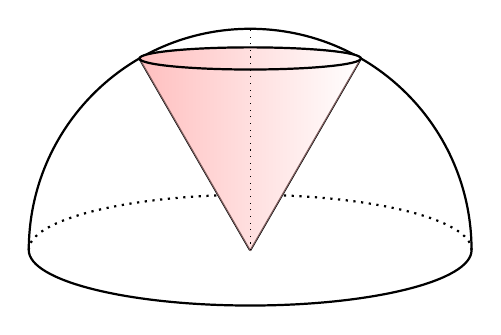
\begin{tikzpicture}
   \draw[thick] (-80pt,0) arc (180:360:80pt and 20pt);
   \draw[dotted,thick] (80pt,0) arc (0:180:80pt and 20pt);
   \draw[thick] (80pt,0) arc (0:180:80pt);
   \draw[thick] (0,0) -- (40pt,69.2820323pt);
   \draw[thick] (0,0) -- (-40pt,69.2820323pt);
   \shadedraw[left color=pink,right color=white, draw=pink!50!black](0,0) -- (40pt,69.2820323pt) arc (0:180:40pt and 4pt) -- cycle;
   \draw[thick] (0,69.2820323pt) ellipse (40pt and 4pt);
   \draw[dotted] (0,0) -- (0,80pt);
  \end{tikzpicture}
 \]
 The design consists of an inverted glass cone of height $h$ and radius $r$ inscribed within a hemisphere of radius $R$.
 \2 Show that the volume of the cone $V = \dfrac{1}{3}\pi(R^2-h^2)h$.\hfill[2]
 \begin{answer}
  Notice that the sloped side of the cone has a fixed length of $R$ and thus, the radius of the cone is given by $\sqrt{R^2-h^2}$ using Pythagoras' Theorem. Using the formula for the Volume of a cone, we get that $V = \dfrac{1}{3}\pi(R^2-h^2)h$.
 \end{answer}
 \2 Given that $R = \sqrt{3}$, find the maximum volume of the cone.\hfill[4]
 \begin{answer}
  We will differentiate twice with respect to $h$ to get our answer.
  \begin{align*}
   \frac{\mathrm{d}V}{\mathrm{d}h}     & = \frac{\mathrm{d}}{\mathrm{d}h}\left[\frac{1}{3}\pi(3-h^2)h\right] \\
                                       & = \frac{1}{3}\pi\cdot\frac{\mathrm{d}}{\mathrm{d}h}(3h-h^3)         \\
                                       & = \frac{1}{3}\pi(3-3h^2)                                            \\
   \frac{\mathrm{d}^2V}{\mathrm{d}h^2} & = \frac{1}{3}\pi(-2h)
  \end{align*}
  When $\frac{\mathrm{d}V}{\mathrm{d}h}=0$, $h=1 \implies  \frac{\mathrm{d}^2V}{\mathrm{d}h^2} = -\frac{2\pi}{3}<0 \implies V$ is at a maximum. This maximum is $\frac{2}{3}\pi$ units$^3$
 \end{answer}

 \1 An inflatable cube is inscribed inside an inflatable sphere such that the cross-section of the figure is as shown: %Question 9
 \[
  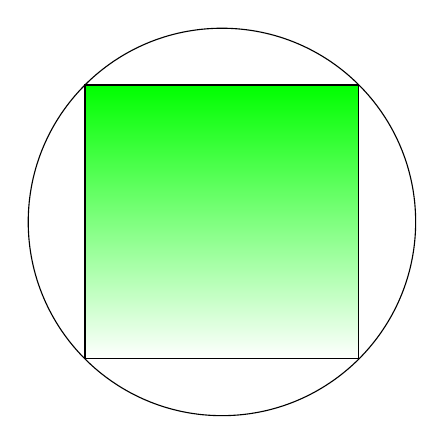
\begin{tikzpicture}
   \draw (0,0) circle (70pt);
   \shade[top color=green,bottom color=white,draw=black] (49.497475pt,-49.497475pt) rectangle (-49.497475pt,49.497475pt);
  \end{tikzpicture}
 \]
 The cube has sides of length 1 unit initially. When the cube is allowed to inflate, the length of its side increase at a rate of $3t$, where $t$ is the time in minutes. As the cube expands, the sphere expands uniformly and bursts when it has a volume of $27\pi$ units$^3$. (The volume of a sphere is given by the formula $V=\frac{4}{3}\pi r^3$ where $r$ is the radius of the sphere)

 \2 Express the length of one of the cube's sides $s$ as a function of time $t$. \hfill[2]
 \begin{answer}
  We are given the fact that $\dfrac{\mathrm{d}s}{\mathrm{d}t}=3t$ so we can see that $s=\frac{3}{2}t^2+C$ where $C$ is $s|_{t=0}=1$
 \end{answer}

 \2 Calculate the time taken for the sphere to burst correct to 3 significant figures. \hfill[3]
 \begin{answer}
  We first have to express the sphere's volume, $V$ in terms of $s$ before getting the value of $t$ from our G.C.
  \begin{align*}
   V          & = \frac{4}{3}\pi \left(\frac{\sqrt{s^2+s^2}}{2}\right)^3      \\
              & = \frac{8\sqrt2\pi}{3}s^3                                     \\
              & = \frac{8\sqrt2\pi}{3}\left(\frac{3}{2}t^2+1\right)^3 = 27\pi \\
   \implies t & = 0.786 \quad\textrm{(From G.C.)}\quad
  \end{align*}
 \end{answer}

 \1 A student set up an experiment as shown below (not drawn to scale):
 \[
  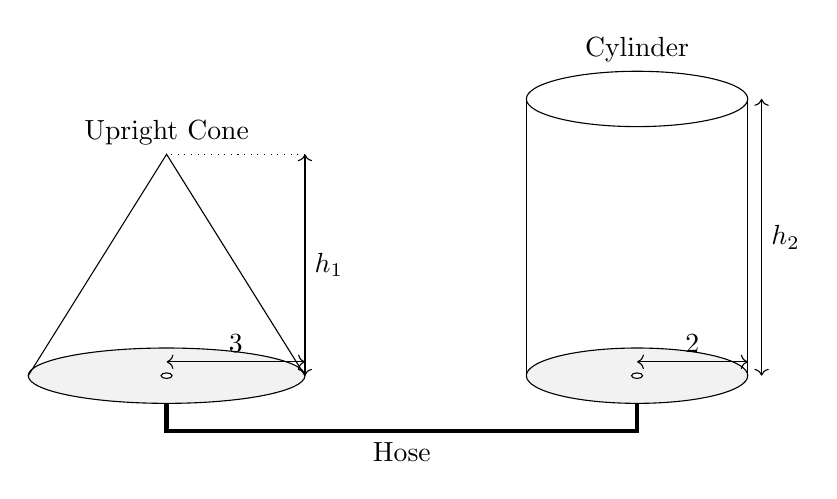
\begin{tikzpicture}
   \filldraw[color=white!90!gray,draw=black] (0,0) ellipse (50pt and 10pt);
   \draw[<->](0,5pt) -- (25pt,5pt) node[above]{3} --   (50pt,5pt);
   \draw[<->](50pt,0pt) -- (50pt,40pt) node[right]{$h_{1}$} --   (50pt,80pt);
   \draw[dotted](50pt,80pt) -- (0,80pt);
   \draw (-50pt,0) -- (0,80pt) node[above]{Upright Cone} -- (50pt,0);
   \draw (130pt,0) -- (130pt,100pt);
   \draw (210pt,0) -- (210pt,100pt);
   \filldraw[color=white!90!gray,draw=black] (170pt,0) ellipse (40pt and 10pt);
   \draw[<->](170pt,5pt) -- (190pt,5pt) node[above]{2} --   (210pt,5pt);
   \draw[<->](215pt,0pt) -- (215pt,50pt) node[right]{$h_{2}$} --   (215pt,100pt);
   \draw (170pt, 110pt) node[above] {Cylinder};
   \draw (170pt,100pt) ellipse (40pt and 10pt);
   \draw[ultra thick] (0,-10pt) -- (0,-20pt) -- (85pt,-20pt) node[below]{Hose} -- (170pt,-20pt) -- (170pt, -10pt);
   \filldraw[color=white,draw=black] (0,0) ellipse (2pt and 1pt);
   \filldraw[color=white,draw=black] (170pt,0) ellipse (2pt and 1pt);
  \end{tikzpicture}
 \]
 The inflatable upright cone and cylinder have fixed plates of radiuses 3 cm and 2 cm  respectively such that only their heights are allowed to vary due to an increase or decrease in volume. The hose is such that gas can be transferred from the upright cone to the cylinder. The gas is incompressible. %Question 10
 \2 Show that $3\dfrac{\mathrm{d}h_{1}}{\mathrm{d}t}+4\dfrac{\mathrm{d}h_{2}}{\mathrm{d}t}=0$.\hfill[2]

 \2 The gas is now being transferred continuously from the cone to the cylinder. Show that the total surface area of the cone and the cylinder is increasing. \hfill[6]

 \1 In a city of Martians, the birth and death rates are high. The population is $x$ Martians (in thousands) and $t$ is the time in years since 2300. The birth rate is 2 times the population per year and the death rate at 1.5 times the square of the population per year. %Question 11

 \2 Show that $\dfrac{{{\textrm{d}}x}}{{{\textrm{d}}t}} = \dfrac{1}{2}(4x - 3{x^2})$\hfill[2]
 \begin{answer}
  The change in population, $\dfrac{{{\textrm{d}}x}}{{{\textrm{d}}t}} =$ Birth Rate $-$ Death Rate
  \begin{align*}
   \frac{{{\textrm{d}}x}}{{{\textrm{d}}t}} = 2x-1.5x^2 =\frac{1}{2}(4x - 3{x^2}) \quad\textrm{(Shown)}\quad
  \end{align*}
 \end{answer}
 \2 Given that, in year 2300, the population was 1000, solve the differential equation in \textbf{(a)}.\hfill[5]
 \begin{answer}
  We will collect like terms on one side and integrate with respect to each variable
  \begin{align*}
   \frac{\mathrm{d}x}{4x-3x^2} = \frac{\mathrm{d}t}{2} ---(1)
  \end{align*}
  Performing Partial Fraction Decomposition,
  \begin{align*}
   \frac{1}{4x-3x^2} = \frac{1}{4x} - \frac{3}{4(3x-4)}
  \end{align*}
  Integrating both sides of (1):
  \begin{align*}
   \frac{1}{4}\ln{|x|} - \frac{1}{4}\ln{|3x-4|} & = \frac{1}{2}t + c                                                 \\
   \ln{\left|\frac{x}{3x-4}\right|}             & = 2t + C                                                           \\
   \left|\frac{x}{3x-4}\right|                  & = \mathrm{e}^{2t+C}                                                \\
   \frac{x}{3x-4}                               & = \pm \mathrm{e}^{2t+C} = \pm \mathrm{e}^{C} \cdot \mathrm{e}^{2t} \\
   \frac{x}{3x-4}                               & = A\mathrm{e}^{2t},\textrm{ letting $A=\pm \mathrm{e}^{C}$}
  \end{align*}
  We now substitute the initial condition $t=0,x=1$ to obtain the value of $A$.
  \begin{align*}
   \frac{1}{-1}   & = A \implies A=-1                             \\
   \frac{x}{3x-4} & = -\mathrm{e}^{2t}                            \\
   x              & = -3x\mathrm{e}^{2t}+4\mathrm{e}^{2t}         \\
   x(1+3e^{2t})   & = 4\mathrm{e}^{2t}                            \\
   x              & = \frac{4\mathrm{e}^{2t}}{1+3\mathrm{e}^{2t}} \\
                  & = \frac{4}{\mathrm{e}^{-2t}+3}
  \end{align*}
 \end{answer}
 \2 Hence, find the population of Martians in the long run.\hfill[2]
 \begin{answer}
  As $t \rightarrow \infty$, $\mathrm{e}^{-2t} \rightarrow 0$. Therefore, $x \rightarrow \dfrac{4}{3}$, i.e. the long run population is $\dfrac{4000}{3}$ Martians.
 \end{answer}

\end{outline}

\end{document}
